\documentclass[dvipdfmx]{jsarticle}
\usepackage[dvipdfmx]{graphicx}
\usepackage{float,listings}

\lstset{
  basicstyle={\ttfamily},
  identifierstyle={\small},
  commentstyle={\smallitshape},
  keywordstyle={\small\bfseries},
  ndkeywordstyle={\small},
  stringstyle={\small\ttfamily},
  frame={tb},
  breaklines=true,
  columns=[l]{fullflexible},
  numbers=left,
  xrightmargin=0zw,
  xleftmargin=3zw,
  numberstyle={\scriptsize},
  stepnumber=1,
  numbersep=1zw,
  lineskip=-0.5ex
}

\begin{document}
\title{数値解析学2 GW中の課題レポート}
\author{19C1123 横尾陸}
\date{\today}
\maketitle

\section*{課題}
微妙に異なる2つの文字列のマッチング
\section{目的}
文字列2行+マッチングを表すoとxの行を出力とするプログラムを作成する.
\section{方法}
この課題に合うようなプログラムを作成する.
  \subsection{提案するアルゴリズム}
\begin{enumerate}
  \item 文字を入力する.
  \item 入力された2つの文字列数を比べる.
  \begin{enumerate}
    \item 文字数が同じだったら1つづつ文字を比べる.
  \end{enumerate}
  \item 多い方に文字数があうように空白を追加する.
  \item 前から順に1文字づつ比べる.
  \item 違う箇所を記憶させておく.
  \item 違う箇所から1文字づつ後ろにずらしていく.
  \item もう1度前から順に比較する.
  \item 文字列とoとxを出力する.
\end{enumerate}
作成したプログラムをListing\ref{huga}に示す.

\begin{lstlisting}[caption=作成したプログラム,label=huga]
#include <iostream>
#include <string>
#include <vector>

class Matching{
private:
  std::string str;
  std::vector<bool> flag;
  bool fl;
  std::string maru, batu;
  int kurikaesi;
  int num;
public:
  Matching()
  {
    maru = 'o';
    batu = 'x';
    num=1;
    fl=false;
  }
  ~Matching()
  {
  }

  std::string input_string()
  {
    std::cout << "string" << num << ":";
    std::cin >> str;
    num++;
    return str;
  }

  void comparison_string_length(std::string &str1, std::string &str2)
  {
    int size = str1.size() - str2.size();
    int num=0;
    fl = (size < 0);

    while(!(str1.size() == str2.size())){
      if(fl){
        str1.push_back(' ');
      }else{
        str2.push_back(' ');
      }
    }
    kurikaesi = str1.size();
    if(fl){
      str1.swap(str2);
    }
    if(size == 0){
      for(int i=0;i<str1.size();i++){
        flag.push_back( str1.at(i) == str2.at(i));
      }
    }else{
      for(int i=0;i<str1.size();i++){
        if(!(str1.at(i) == str2.at(i))){
          num=i;
          break;
        }
      }
      for(int i=str1.size()-1;i>num;i--){
        str2.at(i) = str2.at(i-1);
        str2.at(i-1) = ' ';
      }

      for(int i=0;i<str1.size();i++){
        flag.push_back( str1.at(i) == str2.at(i));
      }
    }
    if(fl){
      str1.swap(str2);
    }
  }

  void output_marubatu(){
    for(int i=0;i<kurikaesi;i++){
      if(flag.at(i)){
        std::cout << maru << " ";
      }else{
        std::cout << batu << " ";
      }
    }
    std::cout << std::endl;
  }

  void output_string(std::string out){
    for(int i=0;i<out.size();i++){
      std::cout << out.at(i) << " ";
    }
    std::cout << std::endl;
  }
};
int main(){
  std::string str1, str2;
  Matching match;
  str1 = match.input_string();
  str2 = match.input_string();

  match.comparison_string_length(str1, str2);

  match.output_string(str1);
  match.output_string(str2);

  match.output_marubatu();

  return 0;
}
\end{lstlisting}

\section{結果}
プログラムを実行した結果です.
\begin{figure}[H]
  \centering
  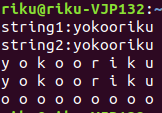
\includegraphics[width=5cm]{images/onaji.png}
  \caption{文字列が同じ場合}
  \label{onaji}
\end{figure}
\begin{figure}[H]
  \centering
  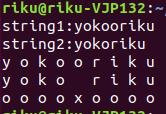
\includegraphics[width=5cm]{images/riku.png}
  \caption{文字列が異なる場合1}
  \label{riku}
\end{figure}
\begin{figure}[H]
  \centering
  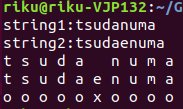
\includegraphics[width=5cm]{images/tsudanuma.png}
  \caption{文字列が異なる場合2}
  \label{tsu}
\end{figure}
図\ref{onaji}は2つの文字列が同じ場合を比較している.図\ref{riku},\ref{tsu}は文字列が異なる場合を比較している.1文字のずれなら比較できていることがわかる.
冗長にはなってしまうがListing\ref{huga}の65行目にListing\ref{hoge}を追加すると2文字のズレにも対応できる.
\begin{lstlisting}[caption=追加するプログラム,label=hoge]
      for(int i=0;i<str1.size();i++){
        if(!(str1.at(i) == str2.at(i))){
          if(num < i){
            num = i;
            fl2 = true;
            break;
          }
        }
      }
      if(fl2){
        for(int i=str1.size()-1;i>num;i--){
          str2.at(i) = str2.at(i-1);
          str2.at(i-1) = ' ';
        }
      }
\end{lstlisting}
図\ref{2moji}は2文字のズレを実行した結果です.
\begin{figure}[H]
  \centering
  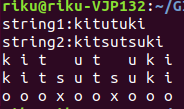
\includegraphics[width=5cm]{images/2moji.png}
  \caption{2文字違う場合}
  \label{2moji}
\end{figure}

\section{考察}
自分のプログラムの書き方が悪いかもしれないが1文字のズレから2文字のズレに対応させるだけでプログラムが長くなってしまう.文字列のズレが増える数だけ対応させようと思ったらそれだけプログラムが長くなってしまうと思う.それを今やっている機械学習を用いたら,文字列のマッチングができるのではないかと考えた.

\end{document}

